\documentclass[11pt]{article}
\pagestyle{plain}

\usepackage{graphicx}
\usepackage{amsmath}
\usepackage{geometry}

\geometry{margin=2cm}

\title{LINMA1170 rapport Devoir 1}
\author{Dallemagne Brieuc - NOMA 77122100}
\date{23/02/2024} 

\begin{document}

\maketitle

\section{Questions théoriques}

\subsection{Question 1}

Démonstration : Soit \( X \in \mathbb{R}^{n \times p} \) on dévellope \( J(X) = \lVert AX - B\rVert^2_F\) :  \( J(X) = \lVert AX - B \rVert^2_F = \text{tr}((AX - B)^T (AX - B)) =
\text{tr}(X^T A^T AX - X^T A^T B - B^T A X^T + B^T B) = \text{tr}(X^T A^T AX - 2X^T A^T B + B^T B) \).(par dévellopement de la norme de Frobénius) En dérivant \( J(X) \) par rapport à \( X \), 
nous obtenons
\[ \nabla J(X) = 2A^T AX - 2A^T B. \]
Donc \( X \) est solution du problème des moindres carrés si et seulement si \( \nabla J(X) = 0 \), le seul moyen d'y parvenir étant que  \( A^T AX = A^T B \). CQFD
\newline
On montre ensuite que ce système admet toujours au moins une solution et qu'elle est unique si \( \text{rang}(A) = n \). 
\newline
Soit \( X \) une solution du problème des moindres carrés. On a alors \( A^T AX = A^T B \). Si \( \text{rang}(A) = n \), alors \( A \) est de rang maximal, donc \( A \) est de plein rang, ce qui implique qu'elle est inversible et qui nous donne donc \( X = (A^T A)^{-1}A^T B \).  \( A \) et \( B \) étant des matrice à valeurs fixées, \( X \) sera unique

\subsection{Question 2}

Démonstration : Nous avons \( A^T AX = A^T B \). par la décomposition QR \( A = QR \), où \( Q \) est une matrice orthogonale et \( R \) est une matrice triangulaire supérieure.
Nous pouvons donc simplifier \( A^T A\) :  \( A^T A = R^T Q^T QR = R^T R \). car \(Q^T Q = 1\) (propriété d'une matrice orthogonale)  ce qui nous donne que \( A^T AX = A^T B \) deviens \( R^T RX = R^T Q^T B \) que on peut encore simplifier en \( RX = Q^T B \). 
Nous arrivons alors un système triangulaire supérieur à résoudre, ce qui est un système facilement résolvable 

\subsection{Question 3}
Démonstration : Nous avons \( m \) points du plan, que nous souhaitons approximer par une courbe paramétrée définie par des B-splines d’ordre 3. L’objectif est de trouver les points de contrôle et les paramètres qui minimisent l’erreur quadratique entre la courbe B-spline et les points donnés.
\newline
Générons les points \( t_i \) donnant \( m \) valeurs uniformément répartie en 0 et 1 . Ensuite définnissons \( n \) points de contrôle \( P^*_j \) et leurs paramètres \( T_j \) selon la méthode proposée dans le document.

\newline
grâces à ces points \( T_j \) nous pouvons trouver nos fonctions B-splines \( B_i(t) \) de degré \( p = 3 \) que nous allons pacer dans une matrice \( A \).
Ce qui nous permet d'avoir un système de type \( AX = B \) (ou \( A \) est la matrice de Bspline et \( B \) les points à approximer).
Nous n'avons plus qu'a appliquer l'algorithme de Least square en passant par la décomposition QR (voir Question 2) pour trouver le \( X \) qui minimisera l'erreur quadratique entres nos points et les Bsplines

\newpage

\section{Évaluation de la complexité temporelle}
Pour la fonction QR j'ai appliqué l'algorithme de Gram-Schmist ce qui m'as donné une complexité de \( O(n^2 \cdot m) \) (voir figure 1,2,3), cette conclusion est basé sur la comparaison de mes résultats par rapport à des fonctions de références qui sont respectivement \(m/10^6\),\(n^2/10^4\) et \(m.n^2/3.10^6\)
et sur l'analyse du code de la fonction qui est composé de 3 boucles for imbriquées (2 allant jusque N et une allant jusque M)




\begin{figure}[h]
  \begin{minipage}[t]{0.5\textwidth}
    \centering
    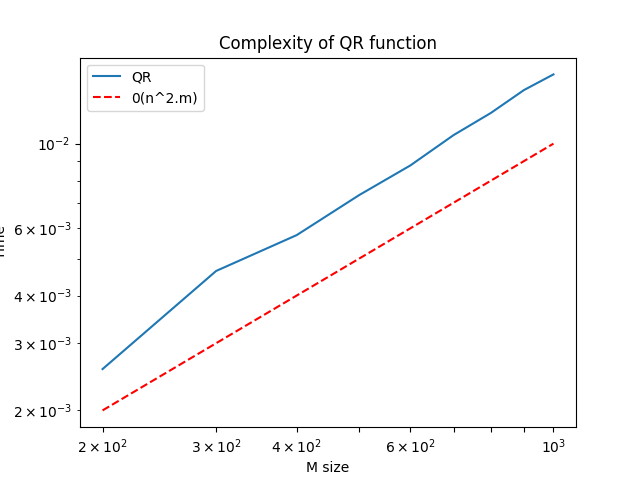
\includegraphics[width=\textwidth]{QR_N100.png}
    \caption{N fixé à 100 et M varie}
    \label{fig:image1}
  \end{minipage}
  \hfill
  \begin{minipage}[t]{0.5\textwidth}
    \centering
    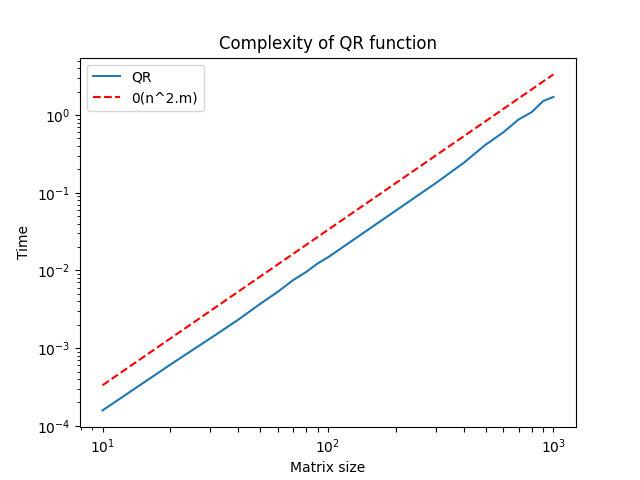
\includegraphics[width=\textwidth]{QR_M1000.png}
    \caption{M fixé à 1000 et N varie}
    \label{fig:image2}
  \end{minipage}
\end{figure}

\begin{figure}[h!]
  \centering
  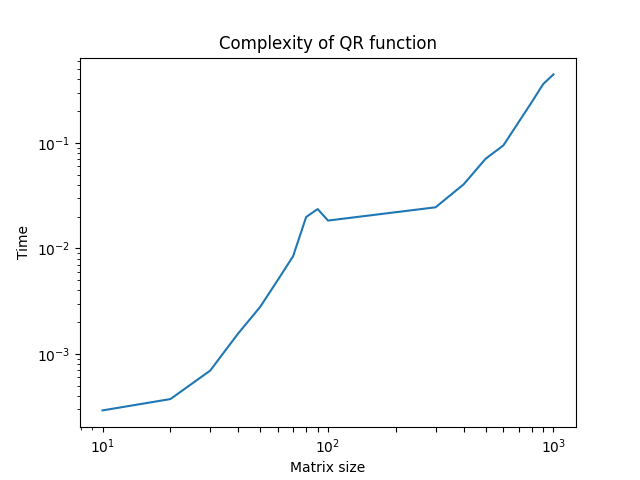
\includegraphics[width=0.7\linewidth]{QR.png}
  \caption{matrice carré}
  \label{fig:3}
\end{figure}




\section{Illustration graphique de l'approximation}
Pour mon exemples je n'ai pas été très originale donc voici Un exemple à la Figure 4, où 573 points ont été approximés par
une courbe en utilisant 40 points de contrôle.

\begin{figure}[h!]
  \centering
  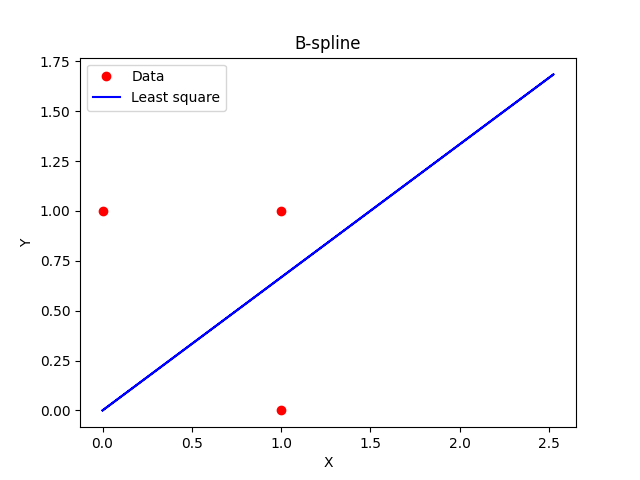
\includegraphics[width=1\linewidth]{Bspline.png}
  \caption{Bspline}
  \label{fig:3}
\end{figure}


\section*{Bibliographie}
\begin{thebibliography}{9}
\bibitem{chatgpt}
  OpenAI,
  \emph{GPT-3.5 Model},
  \url{https://openai.com/gpt-3},
  2022.
(expression mathématiques en latex, aucun réponse n'as été demandé/recopié)

\bibitem{stackoverflow}
  Stack Overflow,
  \emph{Stack Overflow},
  \url{https://stackoverflow.com},
  2008.
  (débuggage)
\end{thebibliography}


\end{document}